\newcommand{\etas}{\ensuremath{\eta_{\mathrm{s}}}}


\chapter{Introduction}


%\section{Microgrid in Background/Perspective}
%\section{What is Microgrid}
In simple terms, a microgrid is a power grid, but on a scale much smaller compared to conventional grid with its distribution system. 
Microgrid usually consists of a small system (distributed system, as opposed to centralized system which we have in place for our main grid.) , complete with its loads (of which there may be some vital loads which must be fed, and other non-vital loads) and some kind of generation capacity. This generation can be conventional - fossil fuel based, like using a microturbine, but ever more increasingly nowadays, also includes generation from renewables like wind and photovoltaics. There may be several other components according to the purpose of the microgrid, and some examples could be batteries and other storage devices, even electric vehicles, other kind of electricity generation systems like fuel cells, tidal energy etc. There may be some new technologies incorporated, like demand response and smart communications etc., and much more relevant to this seminar topic, switches which can cut some lines off/join those with the remaining microgrid (say sectionalizing and tie switches).

%defn given
 
The definition for the microgrid is given as ``A microgrid is a group of interconnected loads and distributed energy resources within clearly defined electrical boundaries that acts as a single controllable entity with respect to the grid. A microgrid can connect and disconnect from the grid to enable it to operate in both grid-connected or island-mode." by U.S. Department of Energy Microgrid Exchange Group\citep{TON201284} and ``Microgrids are electricity distribution systems containing loads and distributed energy resources, (such as distributed generators, storage devices, or controllable loads) that can be operated in a controlled, coordinated way either while connected to the main power network or while islanded." by CIGR\'{E} C6.22 Working Group\citep{CIGRE}.\\
%[https://building-microgrid.lbl.gov/microgrid-definitions]
%explanation (from old report maybe)
Note that there are loads as well as distributed energy resources (conventional or renewable) which can supply at least partly the loads. Due to this aspect, the microgrid is able to island. The U.S. Department of Energy Microgrid Exchange Group definition mentions that the microgrid acts as a single entity with respect to the grid, which just means that the grid only sees the power extracted by the microgrid through the point of common coupling between the main grid / distribution system and the microgrid, and the distribution system operator doesn't have to worry about what is going inside the microgrid, for such operator, microgrid is only a single aggregated load (or if the microgrid is injecting power into the main grid, a source or a negative load). The microgrid operator has to manage the microgrid, dispatching the distributed energy resources in the microgrid, as well as controlling other smart technologies inbuilt in the microgrid, like DSM( Demand Side Management) or reconfiguration etc. The topology/structure will be something like given in figure ~\ref{fig:certs1}. We can see that the microgrid is connected to the main grid via a static switch and PCC (Point of common coupling), so it can be disconnected from the main grid by opening that switch. Another feature we can see is that there are distributed energy resources which can partially/fully feed the loads.
\begin{figure}[tbp]
  \centering
    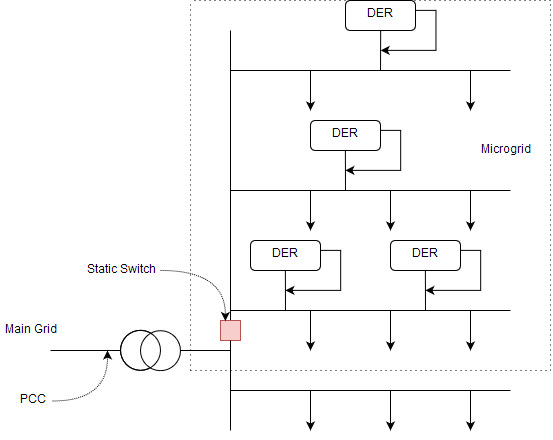
\includegraphics[width=1\textwidth]{MG_Illu.jpg}%paper1gridpaper1grid
    \caption[Microgrid Topology]{An illustrative microgrid topology}
    \label{fig:certs1} 
\end{figure}
%[1.1 of CERTS report]

%control of microgrids - variouslevels, description of each in %certain amount of detail. plus image for the control structure
Now, due to these peculiarities in microgrid, there are certain complexities in the control of microgrid, particularly because it has to be able to operate in islanded mode, isolated from the main grid. This creates several problems. In conventional power systems, the inertia of the system is quite high, because most of the generators are synchronous/rotating machines with high inertia. So conventional power system can deal with power imbalances by using this inertia and see relatively less change in the electrical parameters like voltage magnitude and frequency. However, in microgrid, in islanded mode, power balance is a big issue, because such inertia is simply not there. Even though there are distributed energy resources, they are mostly connected to grid through a power electronic interface, which doesn't offer the inertia similar to a rotating machine, and even if there are a few rotating machines (generators) as the distributed energy resources, they are comparatively much smaller in size and have much lesser inertia compared to their larger counterparts used in the main grids. Apart from acting similar to a slack for microgrid (which makes up for the imbalance of power), the main grid also provides voltage phase frequency and magnitude reference for the microgrid devices and can be generally relied upon to maintain these within specified limits, and there is no requirement of distributed energy resources having to also regulate the voltage magnitude, frequency, etc. This is not the case in islanded mode, however, and finding a control method which will ensure that the voltage magnitude and frequency is within limit is challenging, because the DERs(Distributed Energy Resources), by themselves usually do not have enough inertia to soak up the difference between the desired and actual values as a single DER, and coordinating the control just makes the control system difficult. For example, if we put a PI controller to control the voltage magnitude on two separate DERs, then we may see oscillations due to the competing control. There are usually two options suggested to deal with this. First is to have a decentralized control where a communication system is not needed. This includes having droop control, which doesn't rely on remote measurements and only requires local measurements, eliminating the need for communication between controllers. Most DERs, which are not rotating machines, can be represented by an inverter with filter at the output to suppress high frequency components generated due to switching action (figure~\ref{fig:certs31}).
\begin{figure}[tbp]
  \centering
    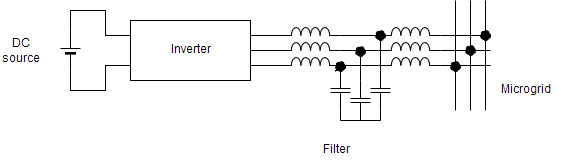
\includegraphics[width=1\textwidth]{DER-inv.jpg}%paper1gridpaper1grid
    \caption[DERs]{A DER connected via inverter to the microgrid}
    \label{fig:certs31} 
\end{figure}
The droop control is generally used in these DERs, and 
%(given in figure ~\ref{fig:certs32})
% \begin{figure}[tbp]
%   \centering
%     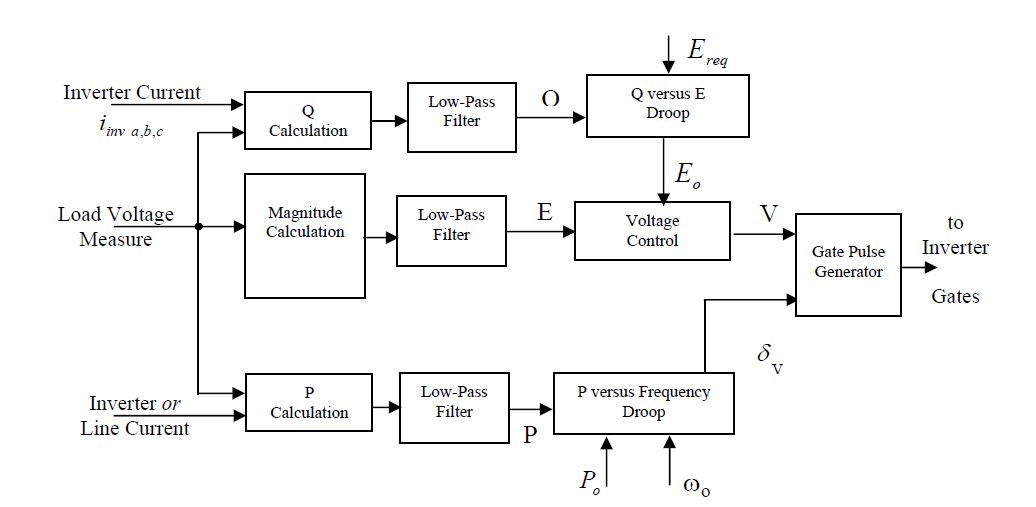
\includegraphics[width=1\textwidth]{certs32.JPG}%paper1gridpaper1grid
%     \caption[Control of DER]{Droop Control of a DER: Control Blocks(image adopted from \cite{CERTS-con})}
%     \label{fig:certs32} 
% \end{figure}
includes $P-f$ and $Q-V$ droops in each of the DERs, and each DER accordingly takes up some of the imbalance of power, resulting in voltage magnitude/frequency deviation. The droop curves (figure ~\ref{fig:00993176})
\begin{figure}[tbp]
  \centering
    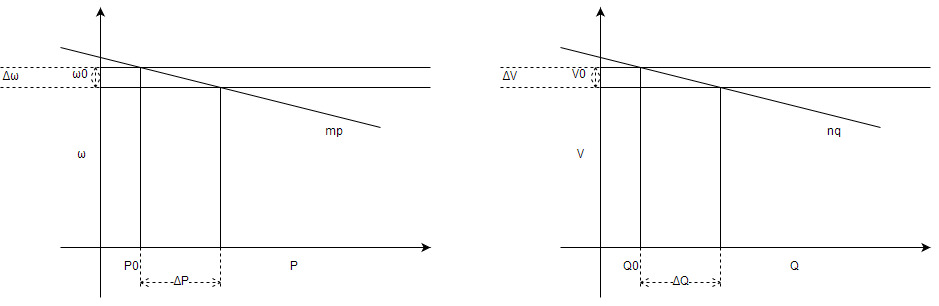
\includegraphics[width=1\textwidth]{Droop_Curves.jpg}%paper1gridpaper1grid
    \caption[Droop Curves]{$P-f$ and $Q-V$ Droop Curves}
    \label{fig:00993176} 
\end{figure}
can give an idea about how droop control works. When the frequency is below the setpoint, according to the droop curve, the real power generation increases, and this helps in bringing the frequency back up, and similarly for the other case and $Q-V$ droop. Now this works very well for real power - frequency droop, but not as much for the $Q-V$ droop, because the reactances of various lines and inductors in the system can cause detection of incorrect voltage levels, and there might be reactive power oscillating between sources. To eliminate this, sometimes a central controller controls all the DERs, loads etc, and gives a particular target to each DER, effectively sharing $P$ and $Q$ imbalance between the DERs. But a central controller requires higher processing power as well as a communication system between the central control system and all the DERs.
Another problem which microgrid operators may face when planning a dispatch etc. is that there is uncertainty in loads, but more importantly, the DERs, especially renewable DERs are quite uncertain, in a way that we can't control how much they generate and it depends on the available sunlight and wind, phenomena which can have very fast fluctuations. So the microgrid has to be able to deal with this uncertainty and absorb the difference via either control of dispatchable DERs, or balancing multiple renewable DERs, or having storage systems, etc.\\
%\section{What is Reconfiguration}	
%reasons for mg optimization - sustainability, efficiency, reliability
There are various reasons to operate a microgrid even though there are certain challenges. For one, it can absorb high amount of renewable DERs without the distribution or transmission system operator having to worry about the local issues. Also, it can be interfaced with many small scale DERs, and efficiently capture as much energy as possible. Due to its small scale, new technologies can easily be integrated into a microgrid, and the system can be operated very efficiently. Another reason to operate a microgrid is that a microgrid has its own DERs, so it is not entirely dependent on the main grid for its operation, and can survive faults and interruptions caused in/by the grid. This creates much more reliable system. These three - sustainability, efficiency, and reliability are why microgrids are used and also how they are operated/planned\citep{mgb05}.
%[refer to mgb 05 and rewrite, and cite it as well]
This usually includes an optimization in order to achieve either of/ some of/ all of these goals in some way.
%different tools available for microgrid optimization
In order to operate this microgrid efficiently and achieve these goals, the operators have various tools at their disposal. These include power exchanged with the main grid, dispatchable DERs, dispatchable loads, storage systems, reconfiguration, and some more depending on the particular cases. Power exchanged with the main grid is unavailable during islanding. While PV (Solar photovoltaic) and wind are generally not considered dispatchable, and we want to utilize maximum energy out of them, other DERs can be dispatchable, such as micro-hydro-turbines, small generators running on fossil fuels, fuel cells, etc. The real as well as reactive power fed by them can be controlled up to a point. Dispatchable loads and DSM can be used to modify the loads or the demand of the system, thus balancing the power generated with the power used, and making the microgrid operation more economical. These schemes may include direct control of the loads by the microgrid operator, or some incentive based scheme where the users are given an option and incentives to perform a certain action. Storage devices can be controlled as well, by controlling their charging-discharging, and there are various options for storage as well.\\
%what is reconfiguration - general idea
Reconfiguration means that we change the network topology itself, not only a-priory but \textit{while} the microgrid is operating as well (\citep{mgrrev01}). Reconfiguration in microgrid is possible due to a large number of lines in microgrids which are tie switches or sectionalizing switches. This can be used in addition to the conventional control variables to achieve better efficiency, lesser costs, lesser losses, more number of loads fed, or any other objective one might want the microgrid to achieve.
%devices involved/operation
This reconfiguration requires presence of tie (normally open) and sectionalizing (normally closed) switches. These enable the microgrid operator to open and close certain lines in the system. The switches can be automatically operated, working on the instructions of the central controller (if such controller exists) or can be operated manually.
%illustrative example
This example provided in \citep{mgrj18} is a very good illustrative example while explaining how reconfiguration takes place (see figure ~\ref{fig:khav1}).
\begin{figure}[tbp]
  \centering
    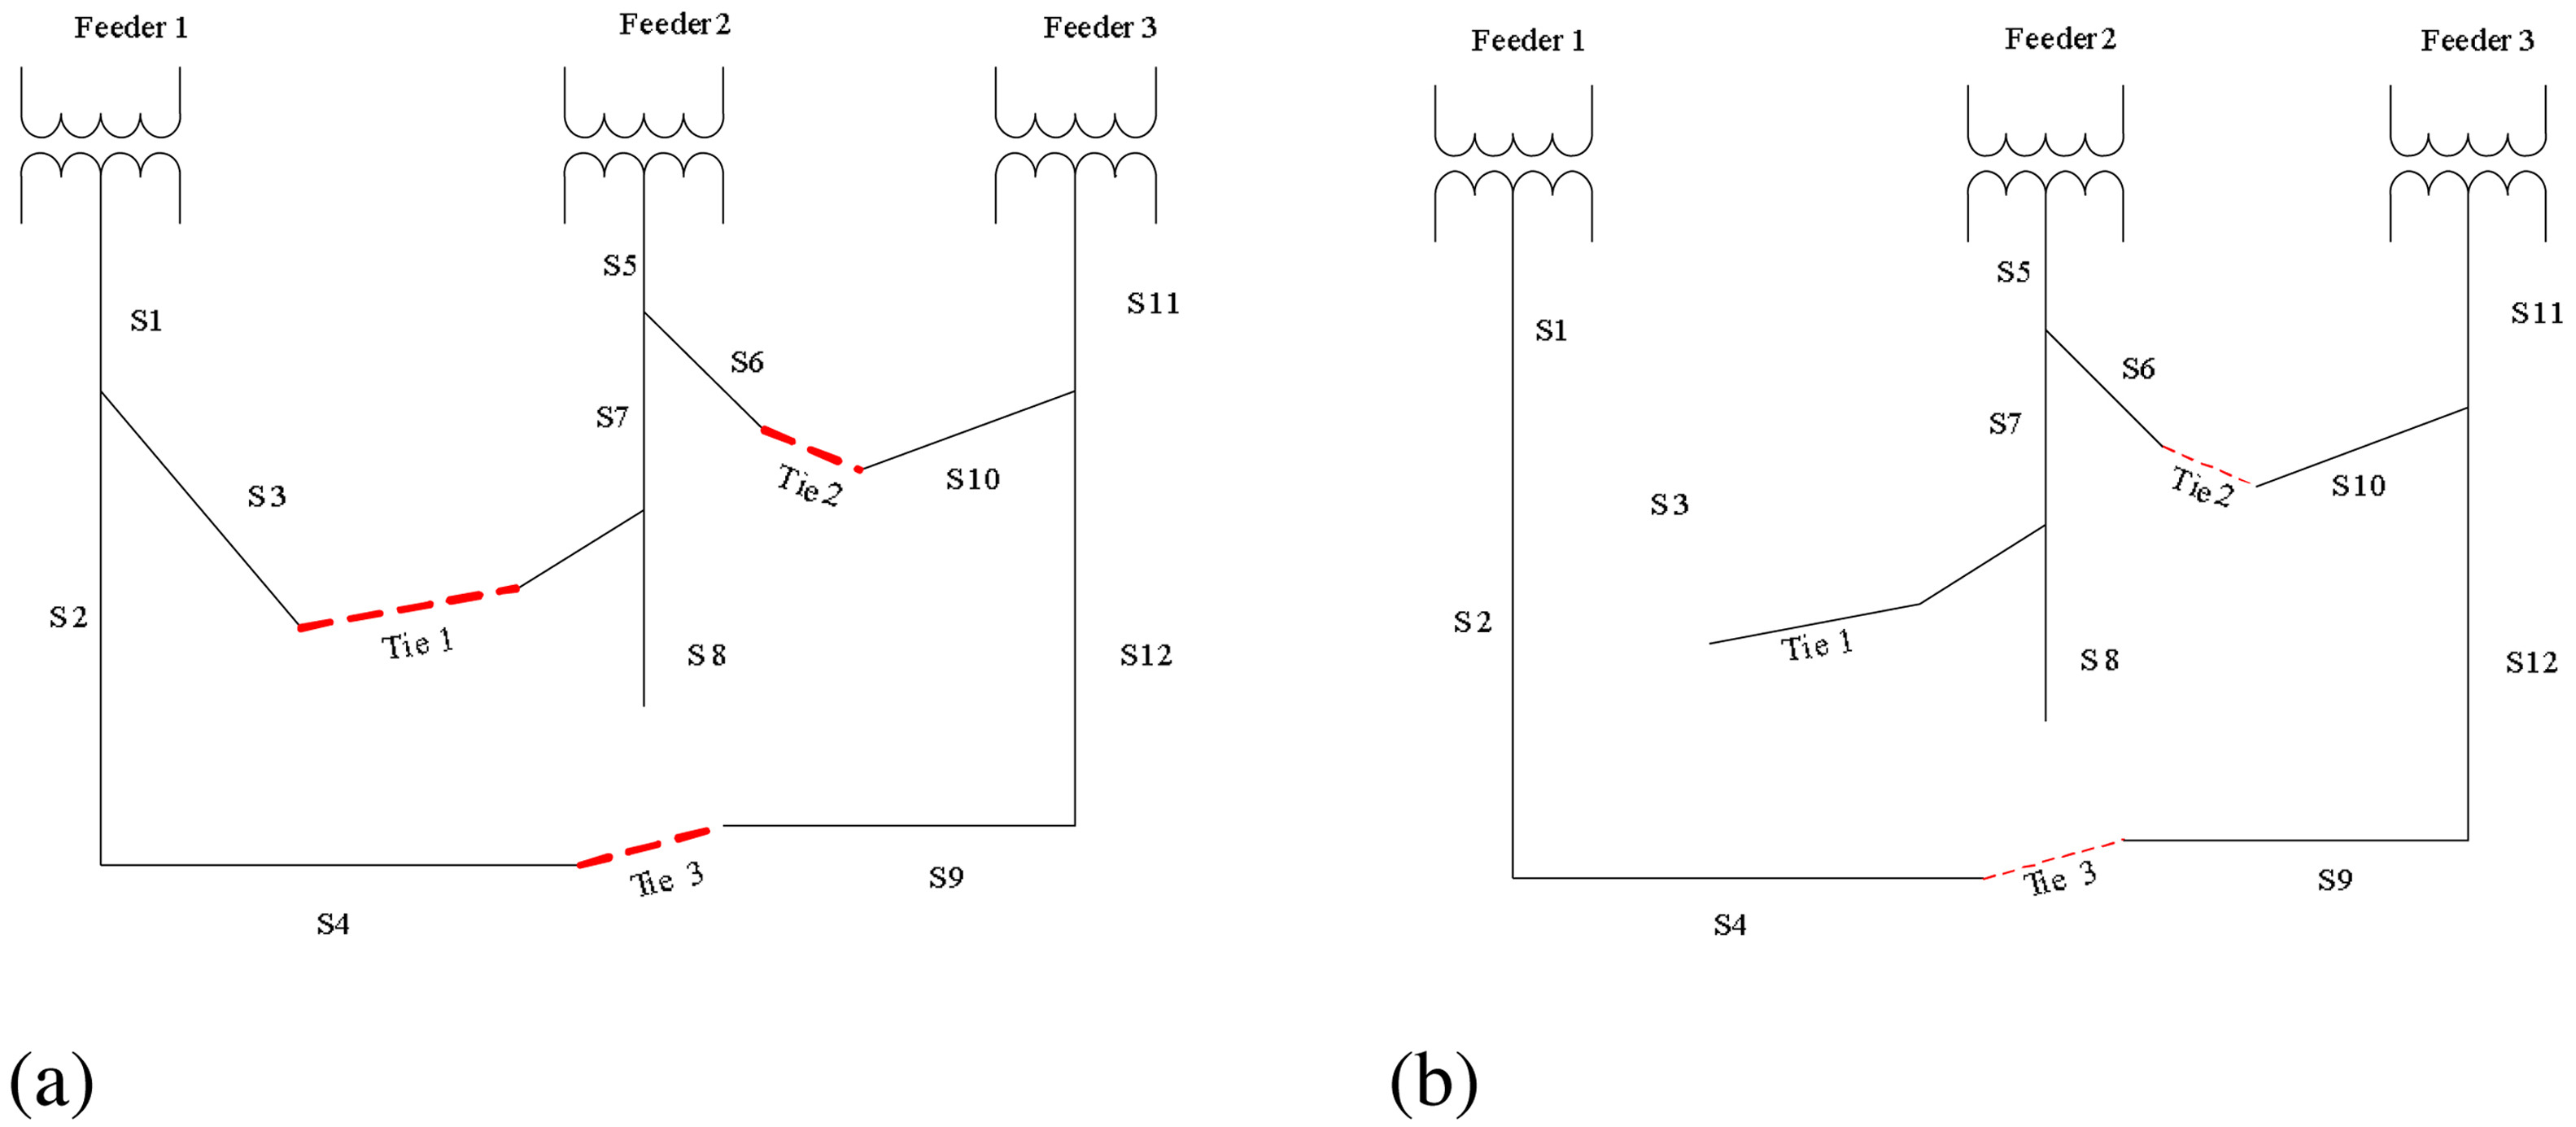
\includegraphics[width=1\textwidth]{khav1.jpg}%paper1gridpaper1grid
    \caption[Reconfiguration]{An illustrative example of reconfiguration(\citep{mgrj18})}
    \label{fig:khav1} 
\end{figure}
In case (a) shown, the initial system is presented. The dotted lines indicate open switches. Now suppose feeder 1 is nearly loaded to its full capacity, and feeder two is quite underloaded, then we might want to shift a load or two on feeder two from feeder 1. We can do this by closing Tie 1 switch and opening S3 switch. Now the load on feeder 1 is a little bit lesser than before, and feeder 2 is a bit more loaded than before. Here the objective was to decrease the load on feeder 1, and since it was a small system with no generation, no PCC to be able to island etc. we could simply choose what to do. As complexity of system increases, choosing when and which switches to operate and which configuration to attain can be quite complicated, but the idea behind reconfiguration is the same.\\
The remaining report presents an exhaustive literature review on the reconfiguration of microgrids, and classifies it, in the chapter ~\ref{ch2}, and concludes in ~\ref{ch4} by stating some of the challenges and future work in the area of microgrid reconfiguration.

%%


%%% Local Variables: 
%%% mode: latex
%%% TeX-master: "../mainrep"
%%% End: 
